%---
\section{Executive Summary}
\label{sec:ExecutiveSummary}

%{\bf \color{red} La parte iniziale del TDR riassume le motivazioni scientifiche e/o tecnologiche che hanno portato alla proposta per la realizzazione del progetto in questione, un’overview della soluzione proposta e l’evoluzione del progetto nel tempo. Si tratta di un sommario esecutivo dalla lunghezza di 1-2 pagine, che include anche una descrizione sommaria dei contenuti del documento.}

\vspace{1cm}

\begin{figure*}[t!]
%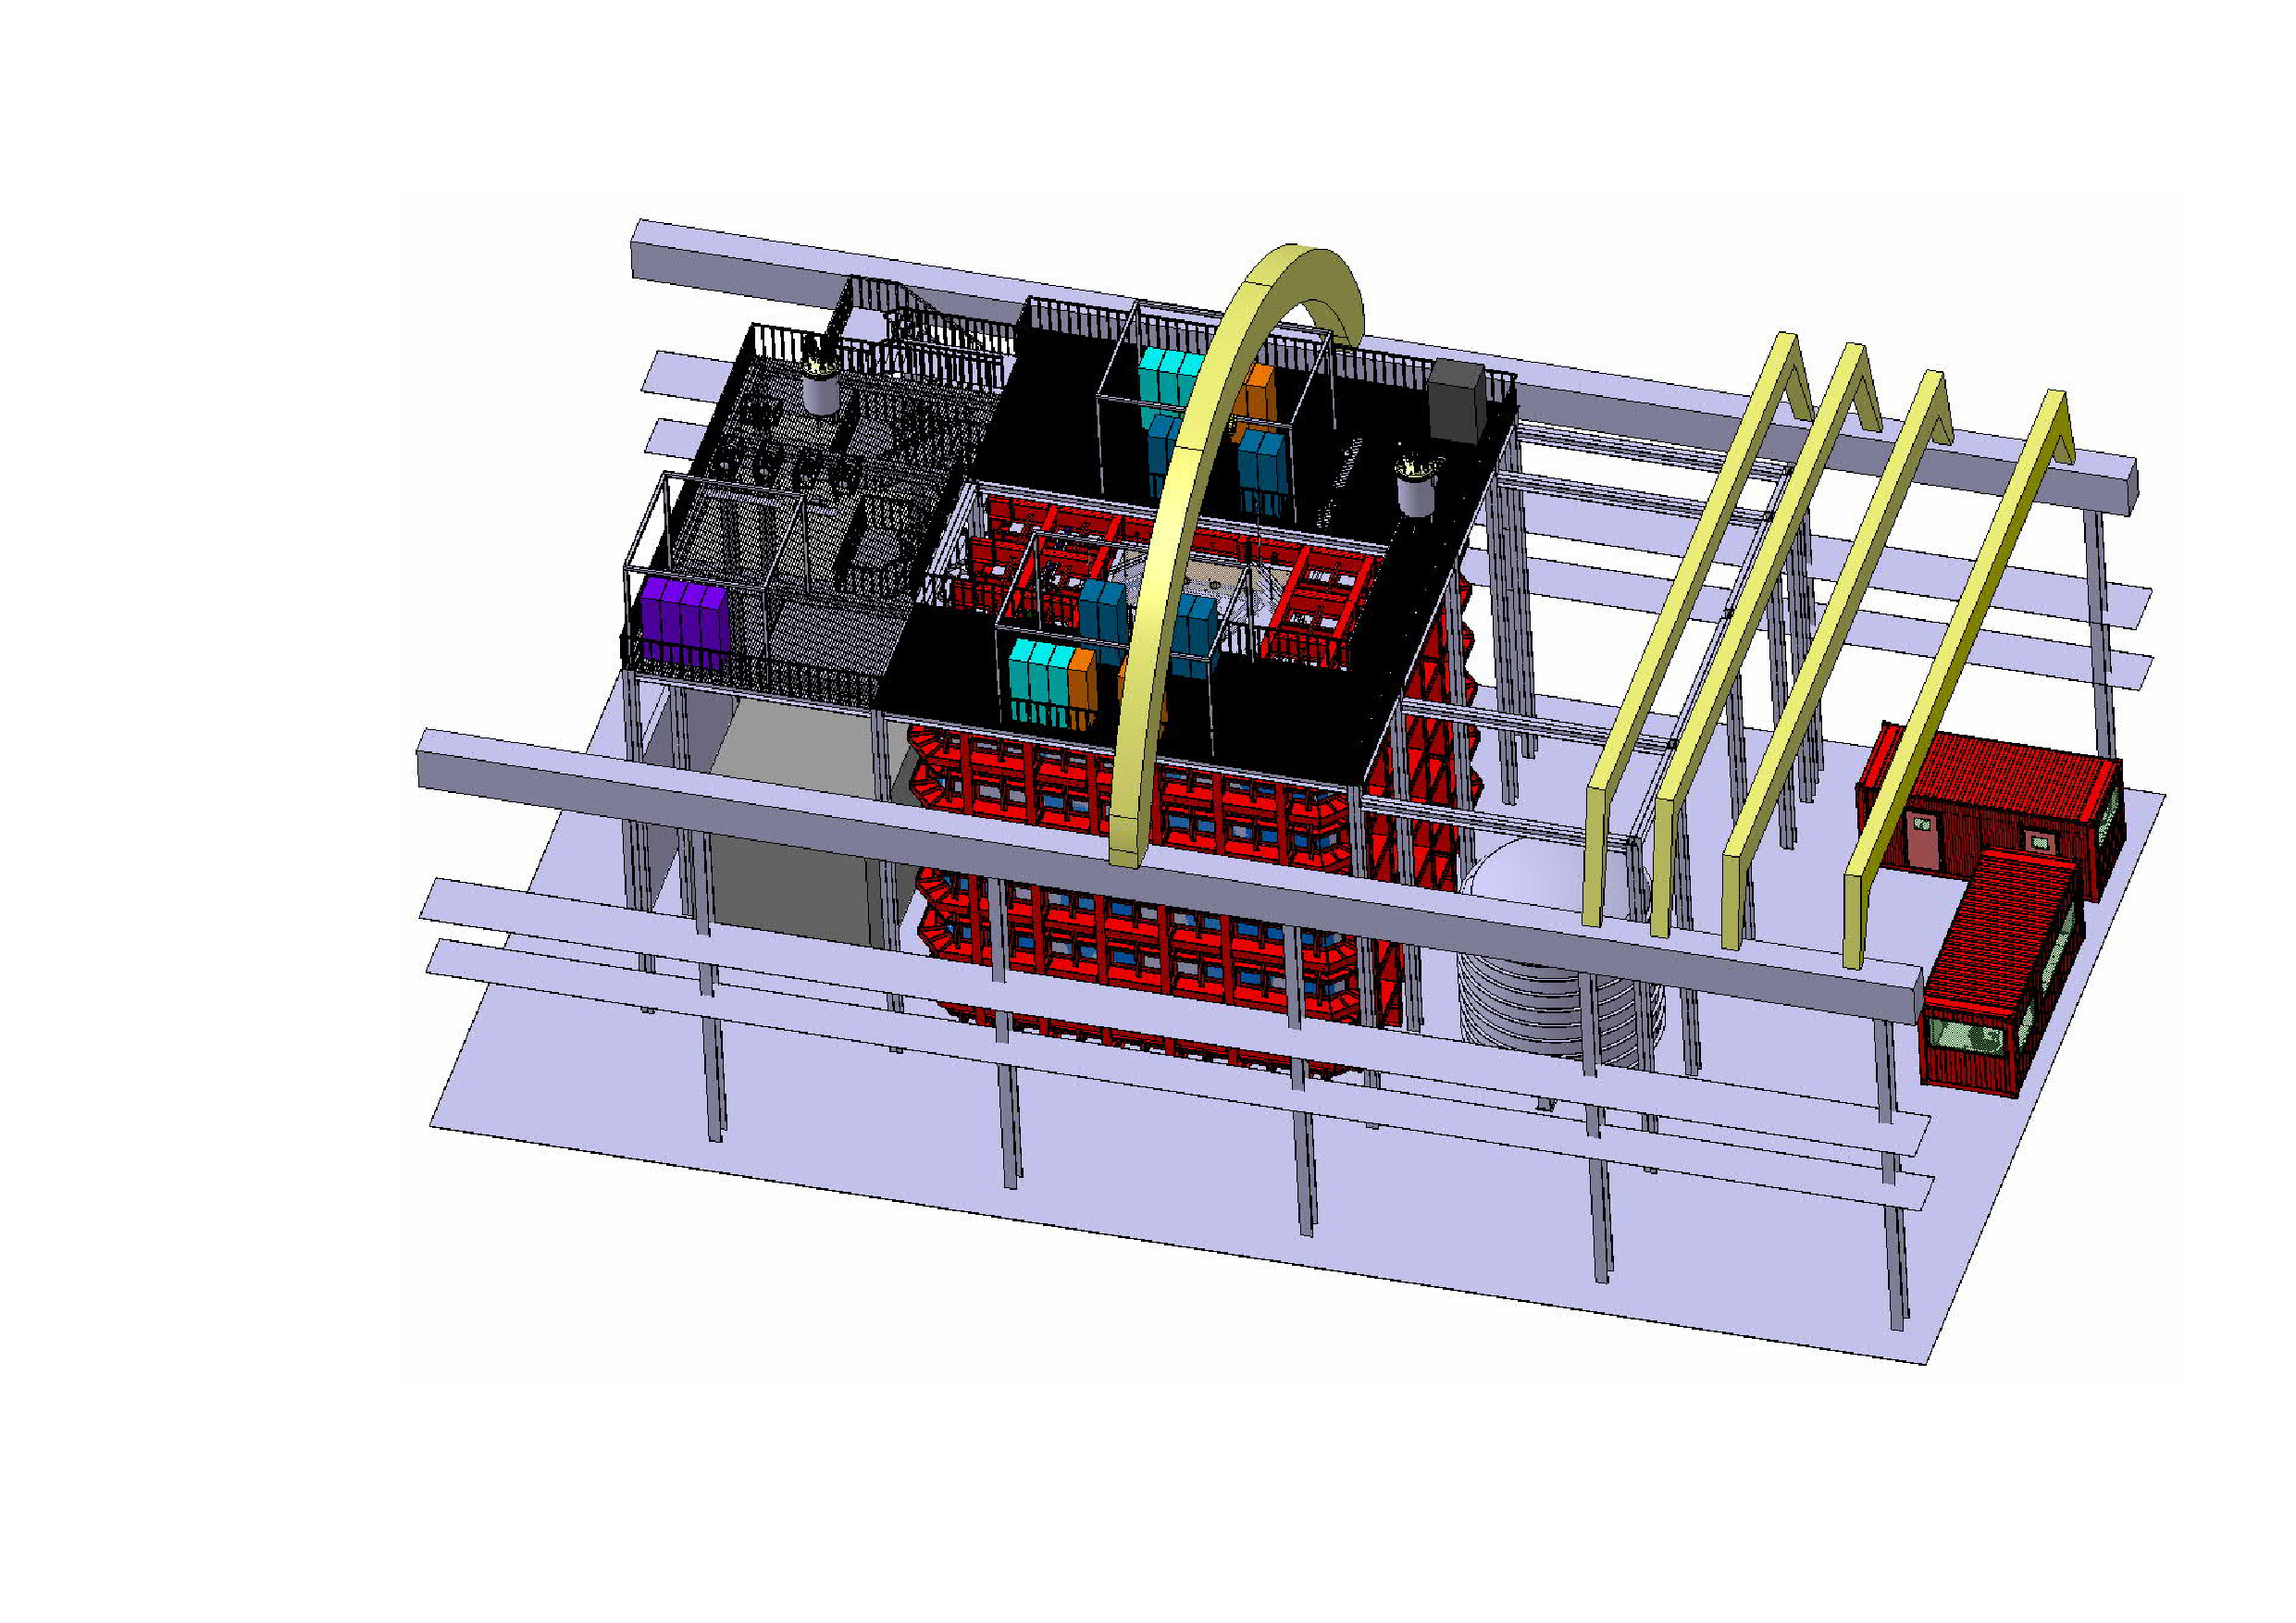
\includegraphics[width=\textwidth]{./Figures/DSk-Overall.pdf}
%\vspace*{-3cm}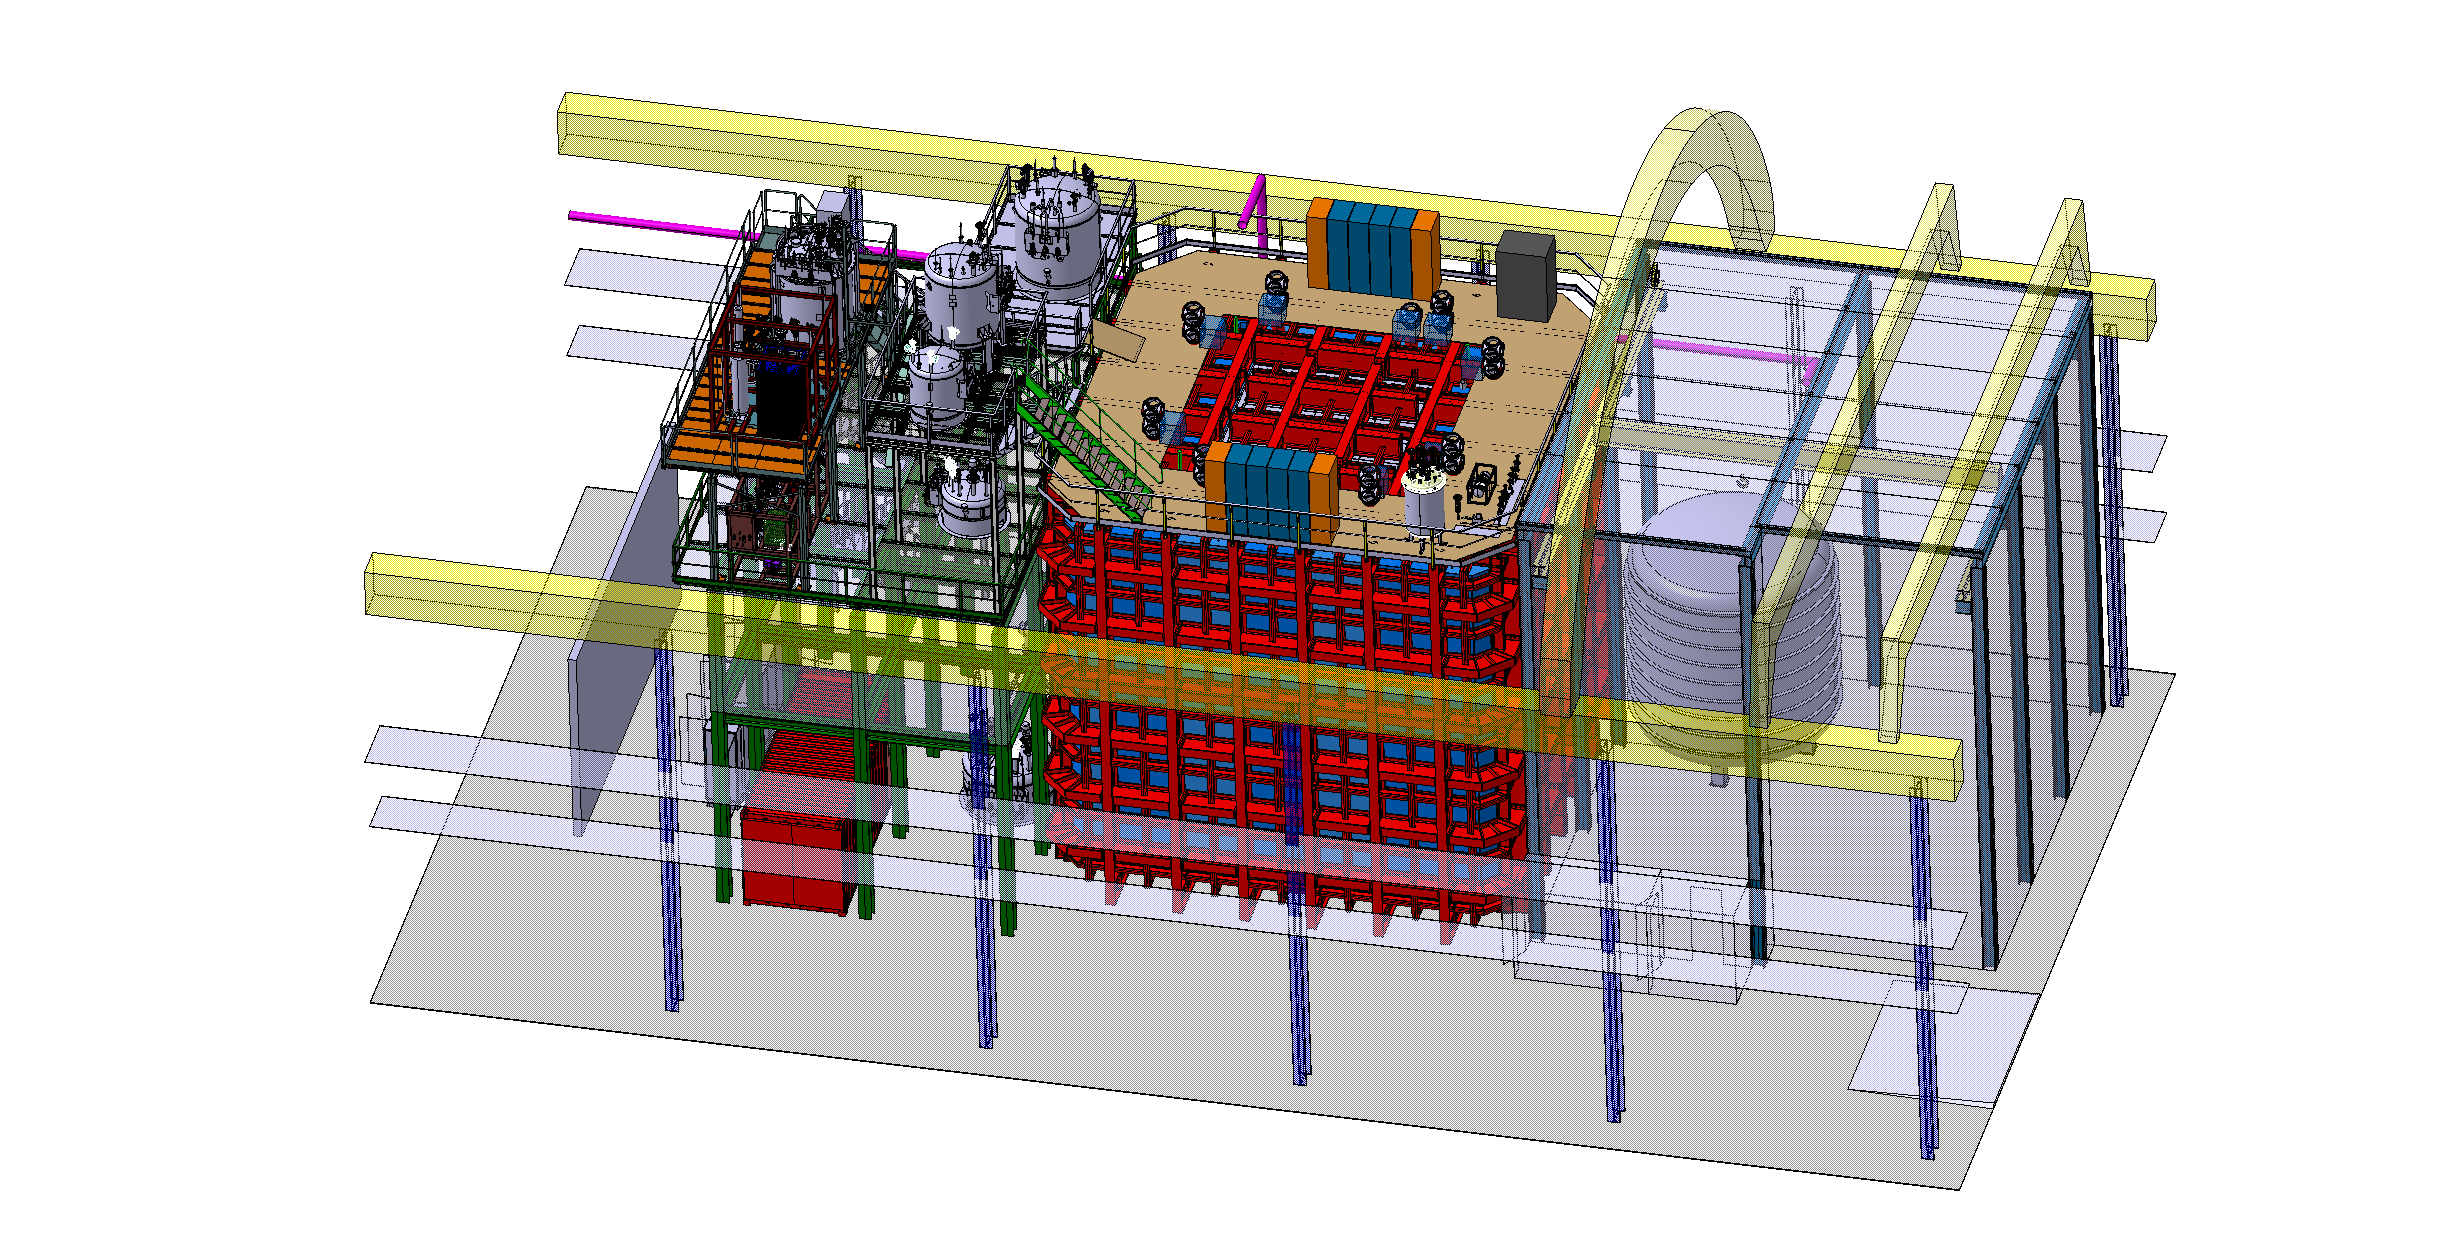
\includegraphics[width=1.5\textwidth, angle=270]{./Figures/assembly_sequence_11_07/58.png}
\vspace*{-3cm}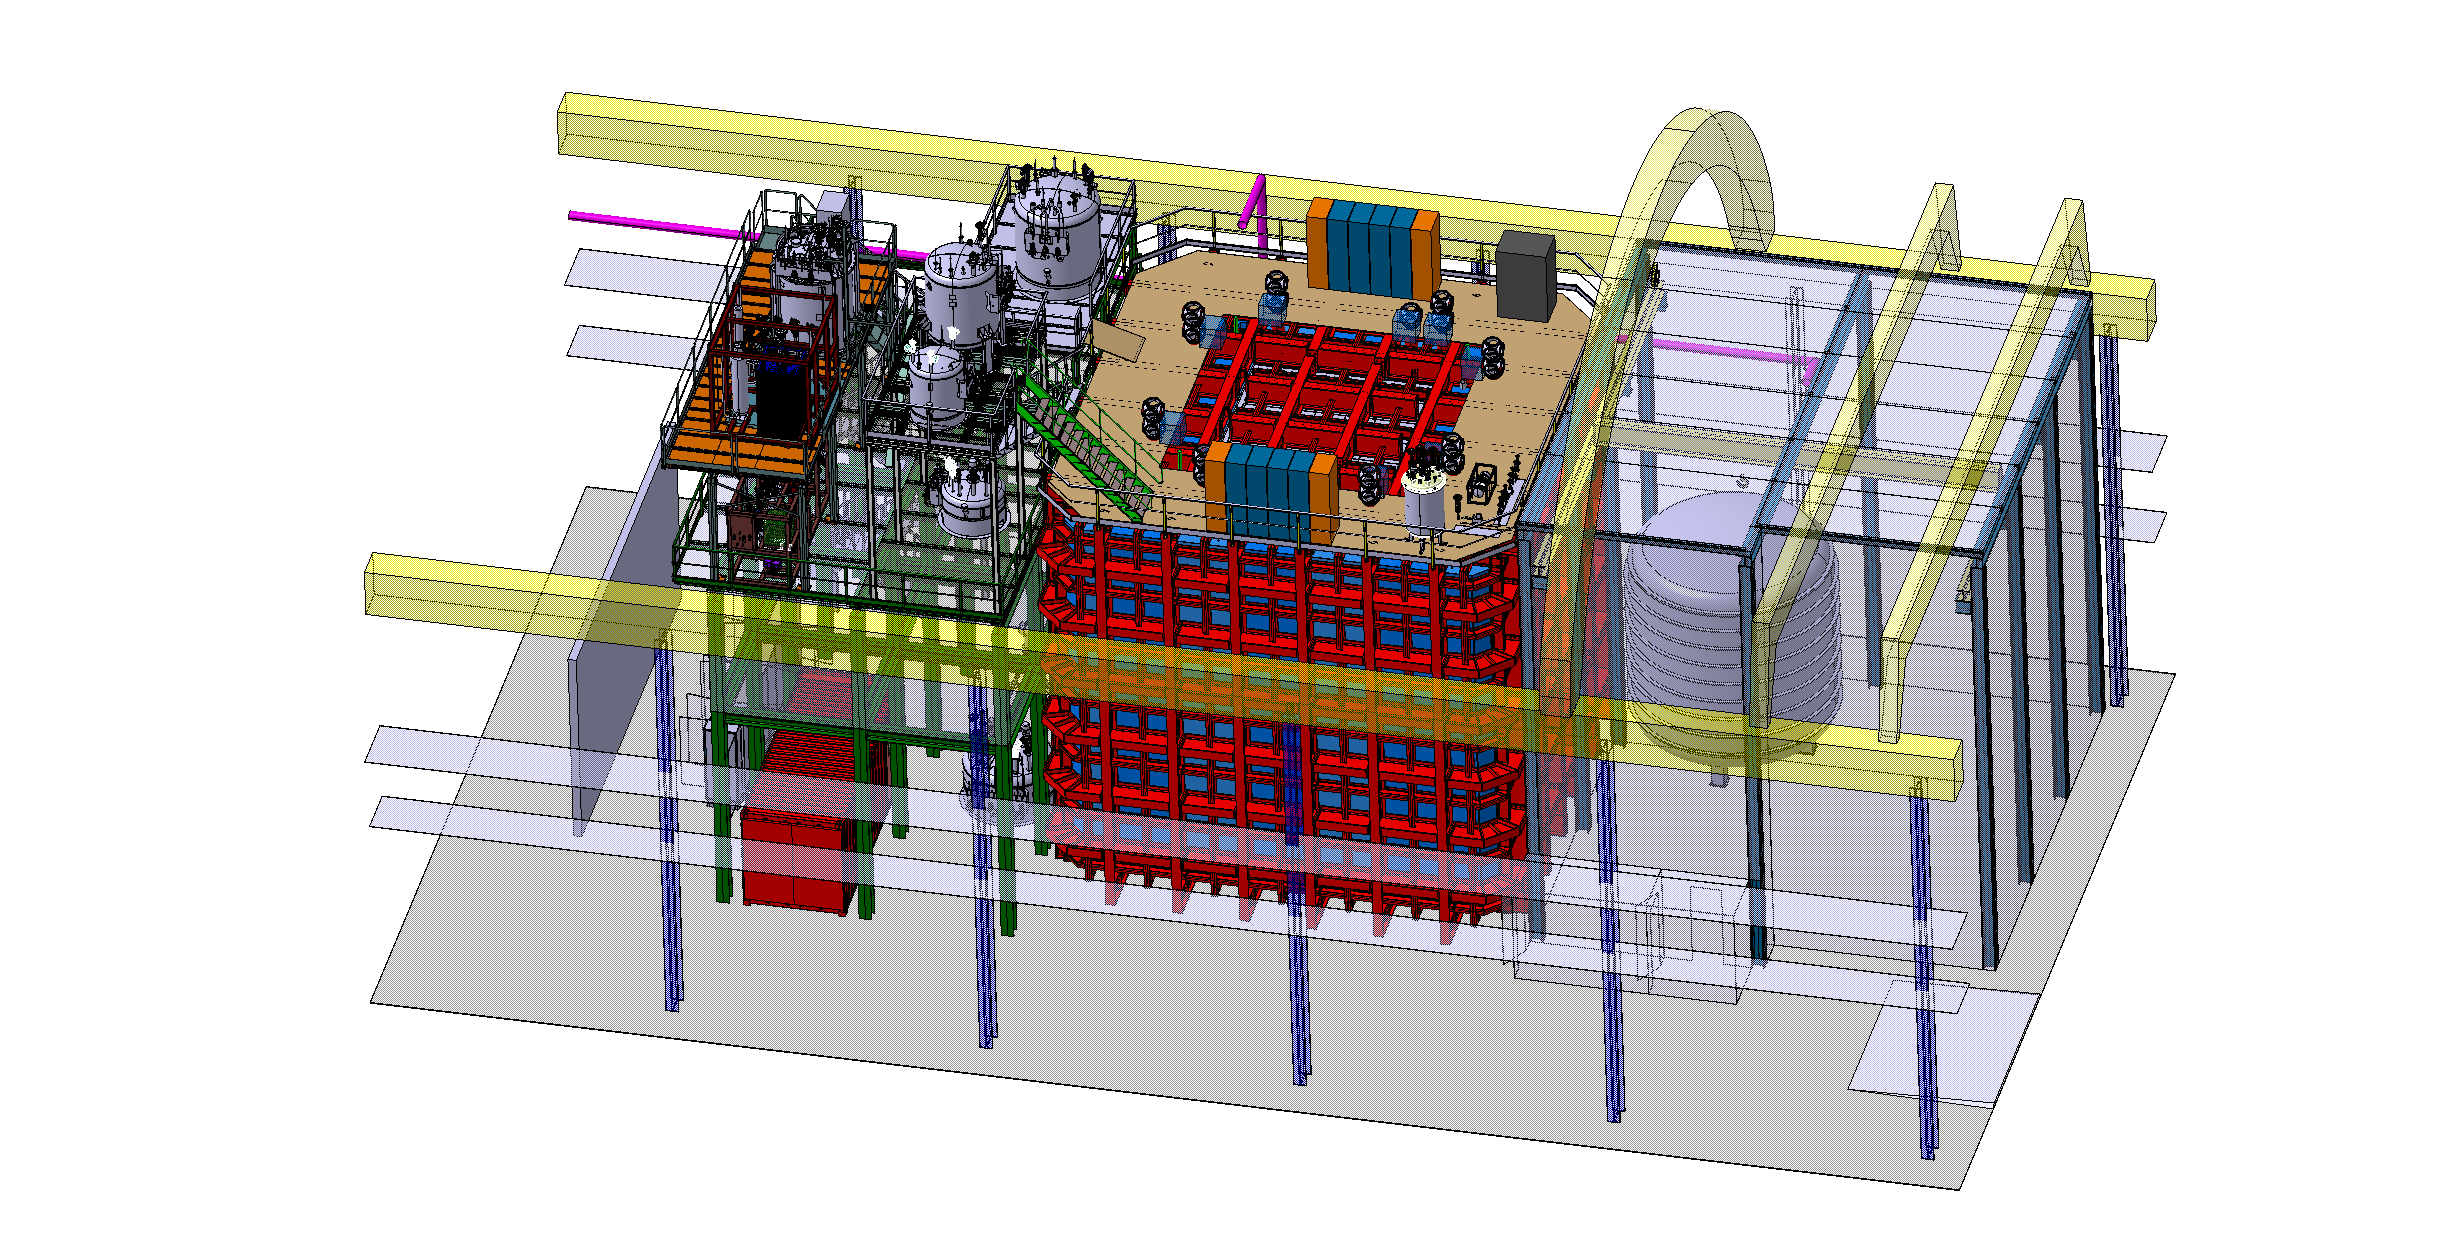
\includegraphics[width=1.5\textwidth, angle=280]{./Figures/assembly_sequence_11_07/58.png}
\caption[Artist rendering of the \DSks\ experiment in Hall C of \LNGS]{Artist rendering of the \DSks\ experiment in Hall\,C of \LNGS.}
\label{fig:Overall-Design}
\end{figure*}

Many fundamental design parameters for the \DSk\ (\DSks) experiment are based on the successful experience of the \DS\ Collaboration in constructing, commissioning, and operating the \DSf\ (\DSfs) detector in a background-free mode. The many technical details of \DSf\ can be found in~\cite{Agnes:2015gu,Agnes:2016cp,Agnes:2016fw,Agnes:2016fz,Agnes:2016tx,Agnes:2017ck,Agnes:2017cl,Agnes:2017cz,Agnes:2017ec,Agnes:2018cn,Agnes:2018dt,Agnes:2018ep,Agnes:2018fg,Agnes:2018ft}.  The \DSks\ liquid argon time projection chamber (\LArTPC) will, too, be deployed at \LNGS\ in the underground Hall\,C, at the center of a newly constructed active veto system.  \reffig{Overall-Design} shows the rendering of the future installation of \DSks\ in the underground Hall~C of \LNGS\ and \reffig{DSk3D} shows an overview of the detailed arrangement of the \LArTPC\ and its anti-coincidence veto detector.  The \DSks\ experiment is designed to operate for a minimum of \DSkExtendedRunTimePlanned\ while maintaining an irreducible background level in the \WIMP\ search region of less than \BackgroundFreeRequirement\ for the total exposure.  To achieve this goal, the design parameters of the \DSks\ experiment have been taken directly from \DSfs, where possible.  Design changes have been made where needed in order to accommodate for the much larger size of \DSks\ and to allow the experimental design to be scalable to a detector at the multi-hundred tonne scale.  In building this preliminary design, issues that have arisen because of design choices or materials selections have been dealt with by limited design modifications, and further optimization will continue as the final development work is completed and a full technical design is made.  

\DSks\ will be built by the Global Argon Dark Matter Collaboration (GADMC) and will consist of two detectors: the inner detector and the veto detector, both hosted in a \pDUNE-like cryostat~\cite{Abi:2017wp,Acciarri:2016wz}.   The inner detector is a \LArTPC\ filled with underground argon (\UAr).  The veto detector is made of a plastic shell, loaded with Gd, surrounding the inner detector, sandwiched between two active atmospheric argon (\AAr) layers.  

%\begin{figure}[t!]
%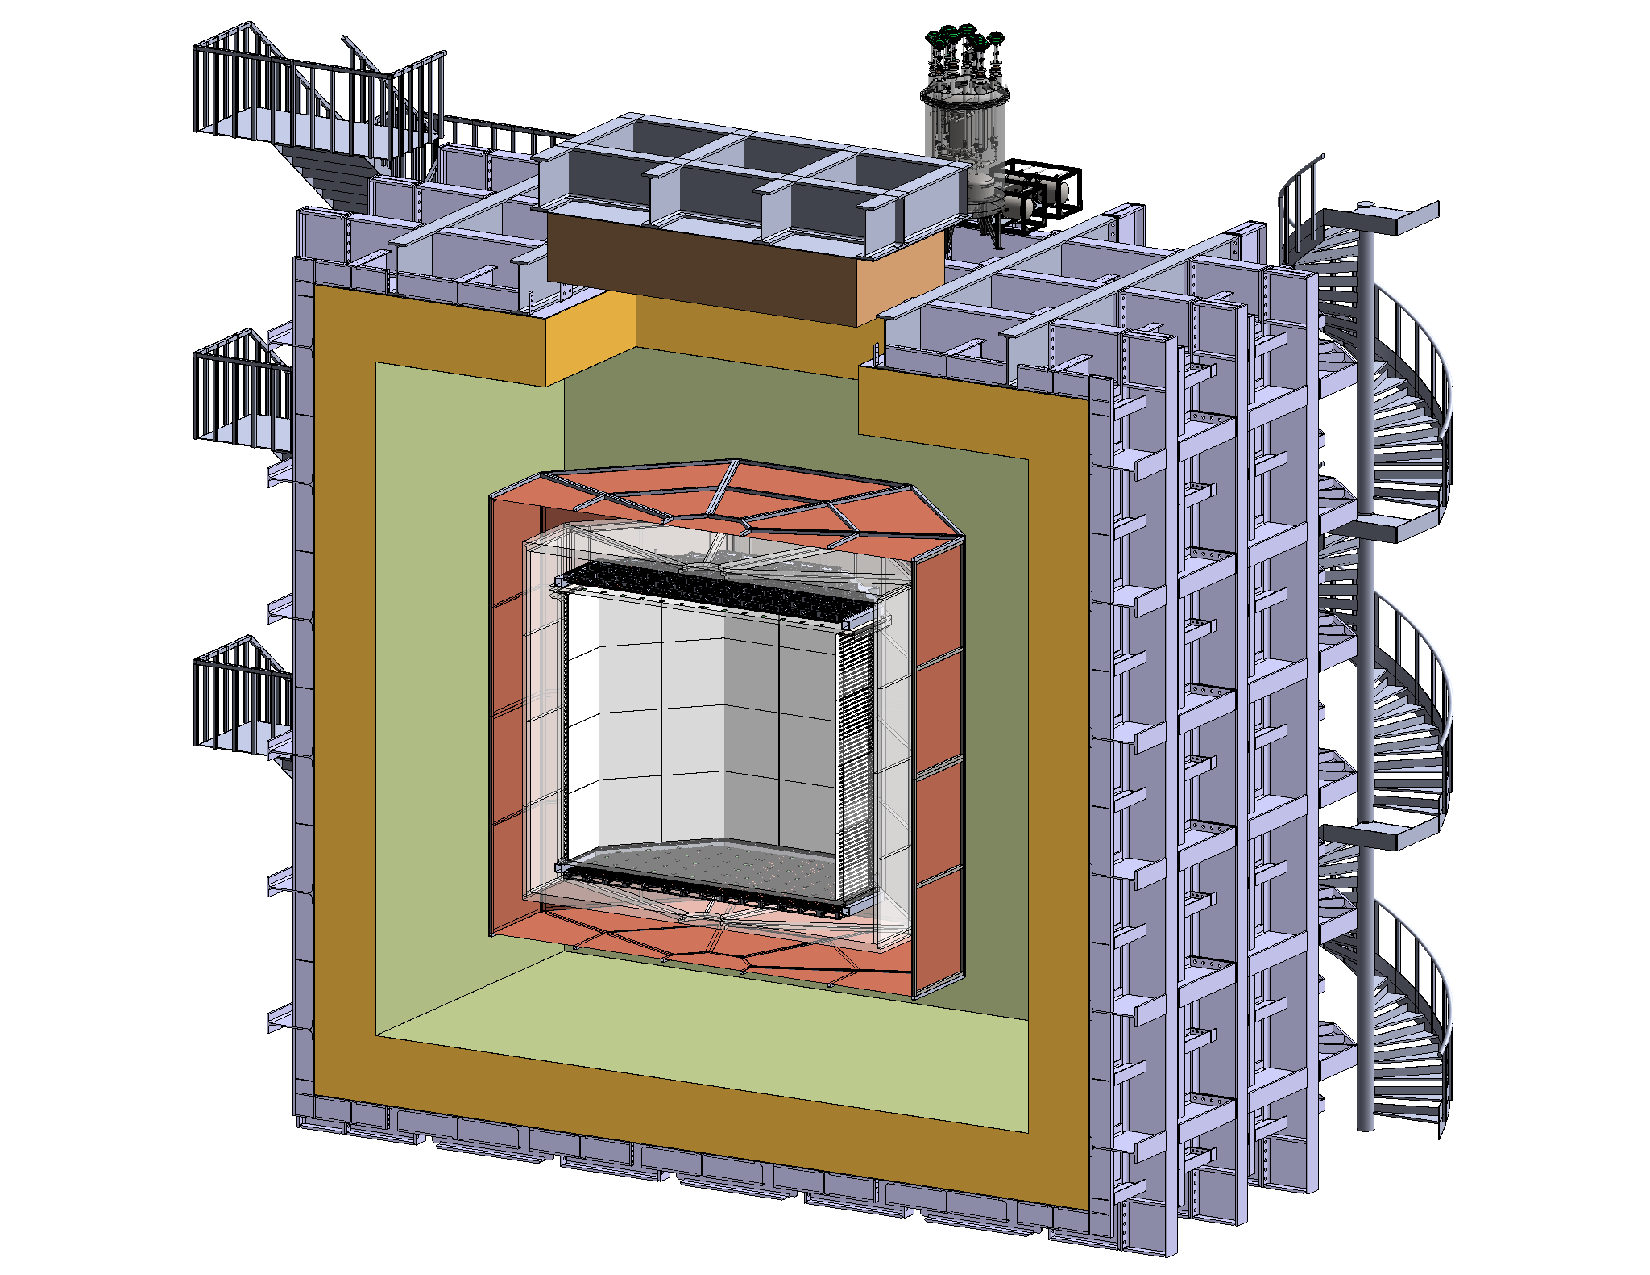
\includegraphics[width=\columnwidth]{Figures/DSk3D.PDF}
%\caption[Artist rendering of the \DSks\ detectors]{Artist rendering of the \DSks\ detectors, with many components omitted for clarity of presentation.  The drawing shows the acrylic (\PMMA) sealed \TPC\  filled with \UAr, surrounded by the veto detector consisting of a \ce{Gd}-loaded acrylic Shell (\GdAS) sandwiched between two atmospheric argon (\AAr) active layers (the Inner Active Buffer, \IAB\ and the Outer Active Buffer, \OAB), all contained in the \pDUNE-like cryostat.  The \OAB\ is optically separated from the rest of the  \AAr\ by a copper vessel.  Technical designs of the support structure of the \TPC\ are already available, and intentionally omitted for clarity of presentation of the main elements.}
%\label{fig:DSk3D}
%\end{figure}

The decision to abandon an organic liquid scintillator veto and to host \DSks\ within a \pDUNE-like cryostat was originally motivated by the need of minimizing the environmental impact on underground \LNGS\ operations, but carries significant performance advantages.  Indeed, operating the \TPC\ directly in the \pDUNE-like cryostat eliminates the need of a cryostat in the immediate proximity of the \UAr\ target, which would significantly contribute to the residual background.  We therefore adopted a new design, with the \UAr-filled \TPC\  immersed in a bath of liquefied \AAr\ held at the same temperature and pressure.  This then allows for the use of a \TPC\ vessel fabricated from the same ultra-pure poly(methyl methacrylate) (acrylic or \PMMA) developed for the \DEAP\ experiment, and thus eliminating the need for a dedicated cryostat or \UAr\ containment vessel. 

% The outer walls of the \TPC\ will sit approximately \SI{2}{\m} away from inner wall of the cryostat.  The \pDUNE-like cryostat may be surrounded by layers of plastic for moderation of cosmogenic and radiogenic neutrons from the rocks surrounding the \LNGS\ Hall\,C, this option is being investigated.

This document, together with the companion documents discussed below, contains all of the information required by the LNGS directorate for the Technical Design Report and is also submitted to the \LNGS\ Scientific Committee in-lieu of the usual semi-annual report. 
All matters related to the project management like detailed budget, funding, project organization as well as a detailed schedule for the overall project are discussed in the attached Project Execution Plan. We also recall that a detailed analysis about health, safety, and environmental issues for which we have contracted an external company to produce a comprehensive Preliminary Risk Assessment (PRA) analysis will be delivered to the LNGS officers as soon as this is available to us.

The present Technical Design Report (TDR) builds upon a similar document submitted in May 2019 for the NSF mid-scale grant, the so-called Intermediate Design Report (IDR), that was made available to LNGS management as well. Few relevant addition to the IDR are included in this TDR, mostly relevant to issues related to the installation in Hall-C and subsequent operation of the \DSks\ experiment.

This TDR addresses first, in Sec.~\ref{sec:PhysicsCase}, the physics motivation and reach for the \DSks\ experiment and the future \LAr\ program envisaged by the \GADMC.  A comprehensive summary of the current design as well as the main results from the past R\&D activities follows in Sec.~\ref{sec:ProjectOverview}. Section~\ref{sec:InstallationAndCommissioning} details the installation phases for the \AAr\ cryostat and the assembly of the TPC and Veto detectors. The required floor space in Hall\,C as well as the technical services that are needed during the installation and the operation of the \DSks\ detector are discussed in Sec.~\ref{sec:TechnicalDesign}. Finally, radiation protection issues related to the handling of the radioactive sources needed for detector monitoring and calibration are briefly discussed in Sec.~\ref{sec:RadioProtection}. 

Having neared completion of the funding for the overall project and finalization of the technical design, our collaboration is planning to start the installation in  Hall\,C in September 2020, provided the needed access, floor plan, and services are granted by \LNGS.  This will allow  to complete the construction phase and begin the commissioning of the \DSks\ detector in the first semester 2023, and reach the frontier in direct detection dark matter searches well in advance that the end of the decade.

